\newpage
\section{Auswertung}
\label{sec:Auswertung}
\subsection{Messung bei einem Druck unter 1 bar}
In der Tabelle \ref{tab:p<1} sind die gemessenen Werte
von der Temperatur des Gases und der Druck
von der ersten Messung, die mit dem Versuchaufbau aus
dem Kapitel \ref{sec:p<1} durchgeführt wurde, aufgetragen.
Der  Umgebungsdruck\footnote{Dieser Wert wurde bei der Messung vergessen zu messen und wird hier nur als 1 bar angenommen.}
 beträgt:
\begin{align*}
p_\mathrm{0}=1\si{\bar}.
\end{align*}
\begin{table}  %Tabelle 1.Messung
  \centering
  \caption{Messwerte die mit Hilfe des Gerätes aus der Abbildung \ref{abb:aufbau1} gemessen wurden, bei einem Druch unter $1\,\si{\bar}$.}
  \label{tab:p<1}
  \begin{tabular}{c c}
    \toprule
    Temperatur des Gas &  Druck \\
    $T_\mathrm{g}/ \si{\kelvin}$ & $p/\si{\bar} $ \\
    \midrule
    307,15 & 0,080\\
    312,15 & 0,105\\
    320,15 & 0,132\\
    321,65 & 0,140\\
    323,65 & 0,150\\
    328,15 & 0,170\\
    330,15 & 0,180\\
    333,15 & 0,200\\
    338,15 & 0,250\\
    342,15 & 0,300\\
    346,15 & 0,350\\
    349,15 & 0,400\\
    352,15 & 0,450\\
    354,65 & 0,500\\
    357,15 & 0,550\\
    359,15 & 0,600\\
    361,15 & 0,650\\
    363,15 & 0,700\\
    365,15 & 0,750\\
    \bottomrule
  \end{tabular}
\end{table}
\FloatBarrier
Werden diese nun in der Form $\log(p/p_\mathrm{0})$ in Abhängigkeit von
$1/T$ aufgeträgen,
lässt sich mit Hilfe der Linearen Regression eine
Ausgleichsgrade bestimmen.
Dies ist in der Abbildung \ref{abb:plot1} dargestellt.
\begin{figure}
  \centering
  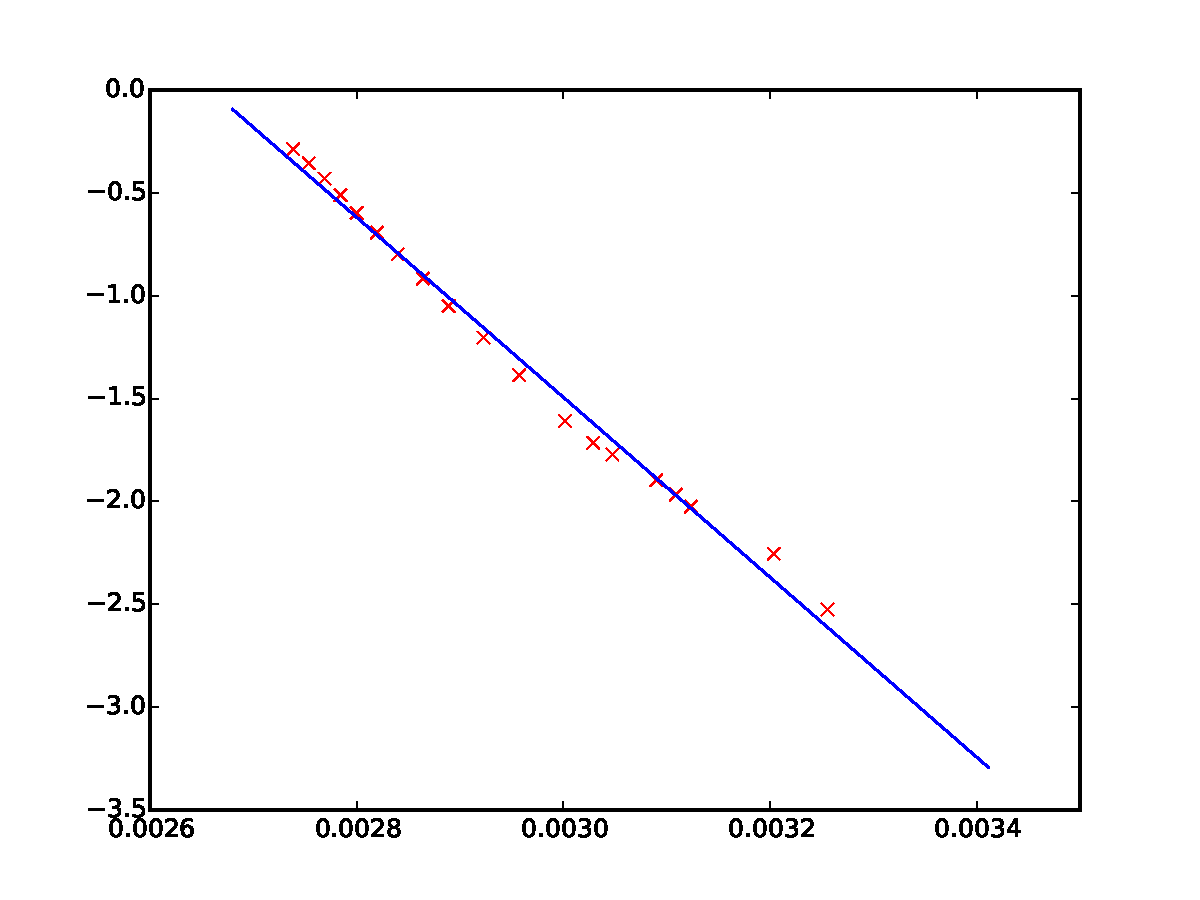
\includegraphics[width=0.7\textwidth]{plot1.pdf}
  \caption{Messwerte aus Tabelle \ref{tab:p<1} die in der Form $1/T_\mathrm{g}$ nach $\log(p/p_\mathrm{0})$ aufgetragen sind.}
  \label{abb:plot1}
\end{figure}
\FloatBarrier
Aus der Linearen Regression ergibt sich für die Parameter:
\begin{align*}
  a=&   11,63\\
  b=&  -4373,84\,\si{\per\kelvin}
\end{align*}
Nun ergibt sich aus der Clausius-Clapeyronschen Gleichung
unter der Annahme, dass $V_\mathrm{F}$ gegen über
$V_\mathrm{D}$ vernächlässigbar ist und  für $V_\mathrm{D}$
die idealen Gasgleichung gilt und $L$ Druck- und
Temperaturunabhängig ist, die folgende Formel:
\begin{align}
  p=&p_\mathrm{0}\exp\left(-\frac{L}{R}\cdot\frac{1}{T}\right).\\
\intertext{Diese wird die Formel nun so verändert:}
\log(p)=& \log(p_\mathrm{0})\left(-\frac{L}{R}\cdot\frac{1}{T}\right).\\
\log\left(\frac{p}{p_\mathrm{0}}\right)=&-\frac{L}{R}\cdot\frac{1}{T}.\\
\intertext{Somit ist das aus der Linearen Regression berechnete Steigung}
b=&-\frac{L}{R}\\
\intertext{und durch umstellen der Gleichung ergibt sich}
L=&-b\cdot R.\\
\end{align}
\begin{align*}
\intertext{Somit ergibt sich für die Verdampfungswärme }
L=(36,4\pm0.8)\cdot 10^3 \,\si{\joule\per\mol}.\\
\intertext{als Literaturwert\cite{L} wird die Verdampfungswärme bei $100\,\si{\degreeCelsius}$ und Normaldruck verwendet.}
L_\mathrm{Lit}= 40,66\cdot 10^3 \,\si{\joule\per\mol}\\
\intertext{Somit weicht der gemessene Wert vom dem Literaturwert nach der Formel \eqref{eqn:abweich} um}
a=18,6 \,\si{\percent}
\end{align*}
ab.
\subsection{Messung bei einem Druck über 1 bar}
Bei dieser Messung ergeben sich die in Tabelle \ref{tab:p>1} aufgelisteten Messwerte für $T_\mathrm{g}$ und $p$.
\begin{table}   % Tabelle 2.Messung
  \centering
  \caption{Messwerte die mit Hilfe des Gerätes aus der Abbildung \ref{abb:p>1} gemessen wurden, bei einem Druch über $1\,\si{\bar}$.}
  \label{tab:p>1}
  \begin{tabular}{c c}
    \toprule
    Temperatur des Gas &  Druck \\
    $T_\mathrm{g}/ \si{\kelvin}$ & $p/\si{\bar} $ \\
    \midrule
    295,15 & 1,00\\
    304,05 & 1,04\\
    316,45 & 1,12\\
    323,15 & 1,18\\
    333,15 & 1,29\\
    344,65 & 1,47\\
    353,15 & 1,65\\
    363,15 & 1,93\\
    373,15 & 2,32\\
    383,15 & 2,84\\
    393,15 & 3,51\\
    403,15 & 4,37\\
    413,15 & 5,47\\
    423,15 & 6,80\\
    433,95 & 8,63\\
    443,15 & 10,5\\
    453,15 & 13,0\\
    463,15 & 16,0\\
    472,15 & 19,4\\
    \bottomrule
  \end{tabular}
\end{table}
\FloatBarrier
$p$ wird nun gegen $T_\mathrm{g}$ aufgetragen, wie in Abbildung \ref{abb:plot2} zusehen, und an die Messwerte wird ein Polynom
der Form
\begin{align*}
p(T)=a\cdot T^3+b\cdot T^2 + c\cdot T + d
\end{align*}
angenährt.
Die Konstanten des Polynoms werden mit scipy eine Erweiterung von Python ausgerechnet. Als Konstanten gegeben sich somit
\begin{align*}
  a =&0,0000058,\\
  b =&-0,0057451,\\
  c =&1,9074059,\\
  d =&-210,6931553.
\end{align*}
\begin{figure}
  \centering
  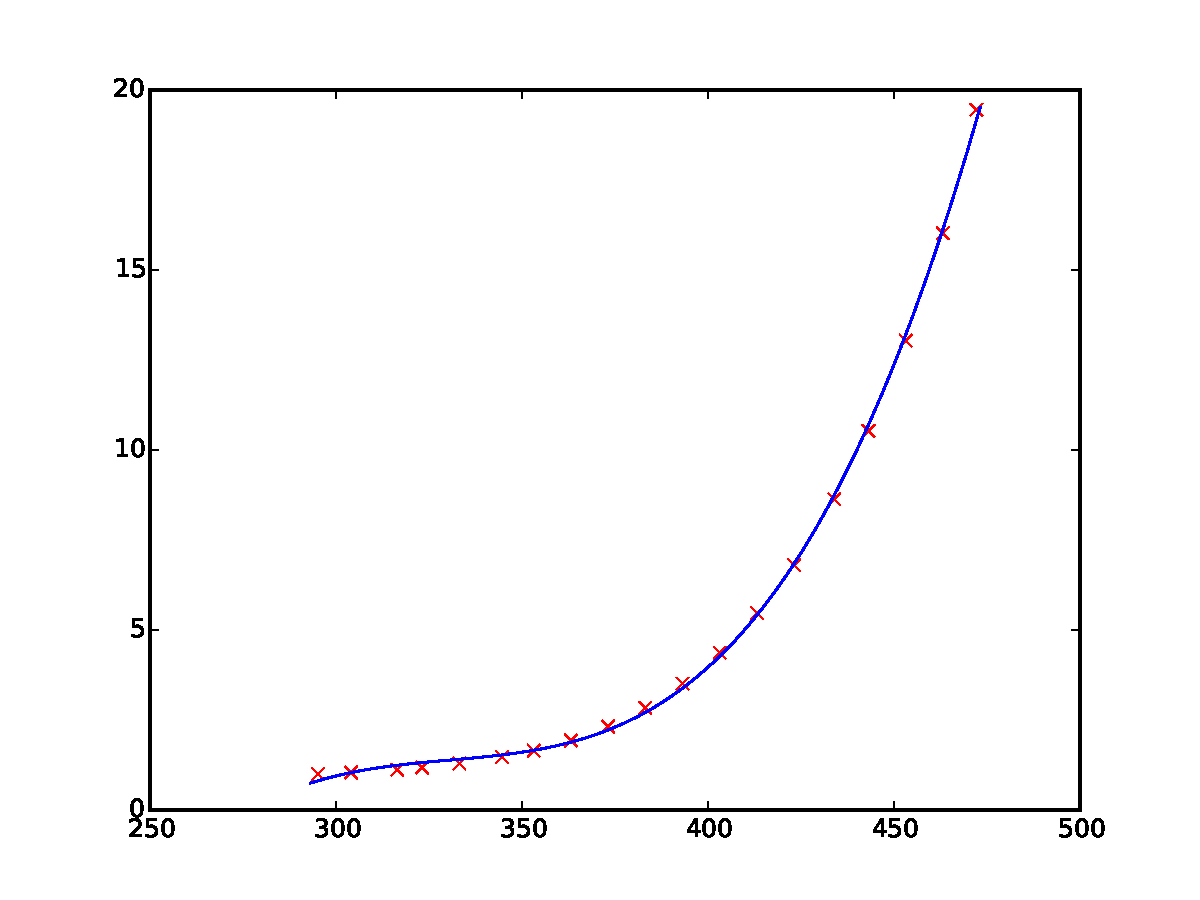
\includegraphics[width=0.7\textwidth]{plot2.pdf}
  \caption{Messwerte aus Tabelle \ref{tab:p>1} die in der Form $T_\mathrm{g}$ nach $p$ aufgetragen sind .}
  \label{abb:plot2}
\end{figure}
\FloatBarrier
Um wieder die Verdampfungswärme $L$ zu berechene,
wird wieder die Clausius-Clapeyronsche Gleichung
verwendet. Da bei der Messung der kritische Punkt überschritten
wird, kann $L$ nicht mehr als konstant angenommen werden.
Trotzdem kann, wie schon bei der Messung unter einem Bar,
$V_\mathrm{F}$ gegen über $V_\mathrm{D}$ vernachlässigt werden.
Jedoch gilt für $V_\mathrm{D}$ nicht mehr die Allgemeine
Gasgleichung sondern die Näherung:
\begin{align}
\left(p+\frac{a}{V_\mathrm{D}^2}\right)\cdot V_\mathrm{D}=R\cdot T \; \; \; \text{mit} \;\; a=0,9\,\si{\joule\cubic\meter\per\mol\tothe{2}}\\
\intertext{Diese Näherung nach $V_\mathrm{D}$ umgestellt ergibt:}
V_{\mathrm{D\pm}}=\frac{RT}{2p}\pm\sqrt{\left(\frac{RT}{2p}\right)^2-a}.
%V_{mathrm{D-}}=\frac{RT}{2p}-\sqrt{\left\frac{RT}{2p}\right)^2-a}
\end{align}
wobei nun zwischen $V_\mathrm{D+}$ und  $V_\mathrm{D-}$ unterschieden werden muss.
Wird nun die Clausius-Clapeyronsche Gleichung nach $L$ umgestellt, ergibt sich:
\begin{align}
L&=V_\mathrm{D\pm}\cdot \frac{\delta p}{\delta T} \cdot T.\label{eqn:L}\\
\intertext{Für die Gleichung muss folglich noch die Ableitung von p bestimmt werden:}
p'(T)&=3a\cdot T^2+ 2b\cdot T + c.
\end{align}
\begin{align}
\intertext{Nun wird alles in die Gleichung \eqref{eqn:L} eingesetzt und es ergeben sich zwei Gleichungen für die Verdampfungswärme:}
L_-=\frac{RT}{2(a\cdot T^3+b\cdot T^2 + c\cdot T + d)}-\sqrt{\left(\frac{RT}{2(a\cdot T^3+b\cdot T^2 + c\cdot T + d)}\right)^2-a} \cdot (3a\cdot T^2+ 2b\cdot T + c )\cdot T\label{eqn:L-}\\
L_+=\frac{RT}{2(a\cdot T^3+b\cdot T^2 + c\cdot T + d)}+\sqrt{\left(\frac{RT}{2(a\cdot T^3+b\cdot T^2 + c\cdot T + d)}\right)^2-a} \cdot (3a\cdot T^2+ 2b\cdot T + c)\cdot T.\label{eqn:L+}.
\end{align}
Diese Gleichungen der Verdampfungswärme werden nun in Abhängigkeit
von der Temperatur aufgetragen wie in den Abbildungen \ref{abb:-} und \ref{abb:+}
zusehen.


\begin{figure}
  \centering
  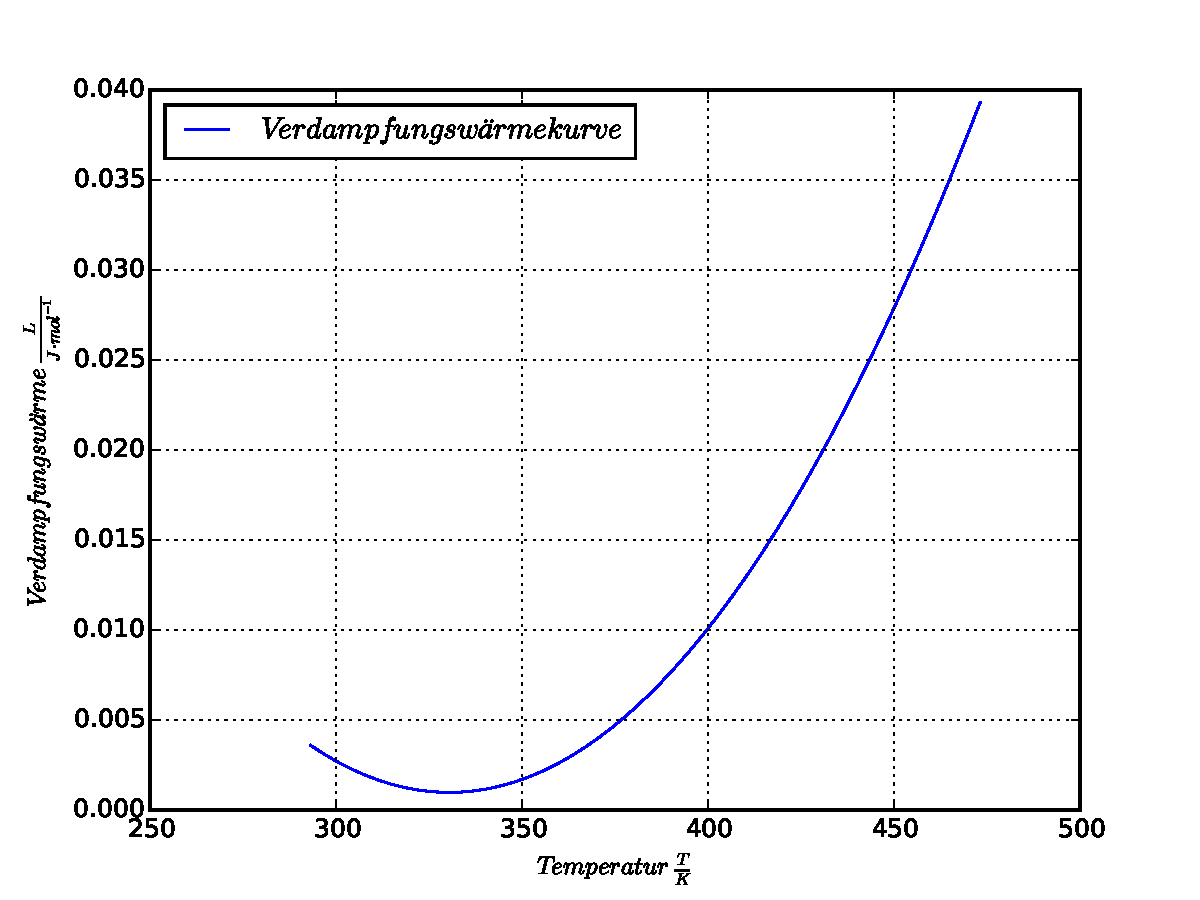
\includegraphics[width=0.7\textwidth]{plot3.pdf}
  \caption{Verdampfungswärme $L$ in Abhängigkeit von $T$ aus der Formel \eqref{eqn:L-}mit negativem Vorzeichen vor der Wurzel.}
  \label{abb:-}
\end{figure}

\begin{figure}
  \centering
  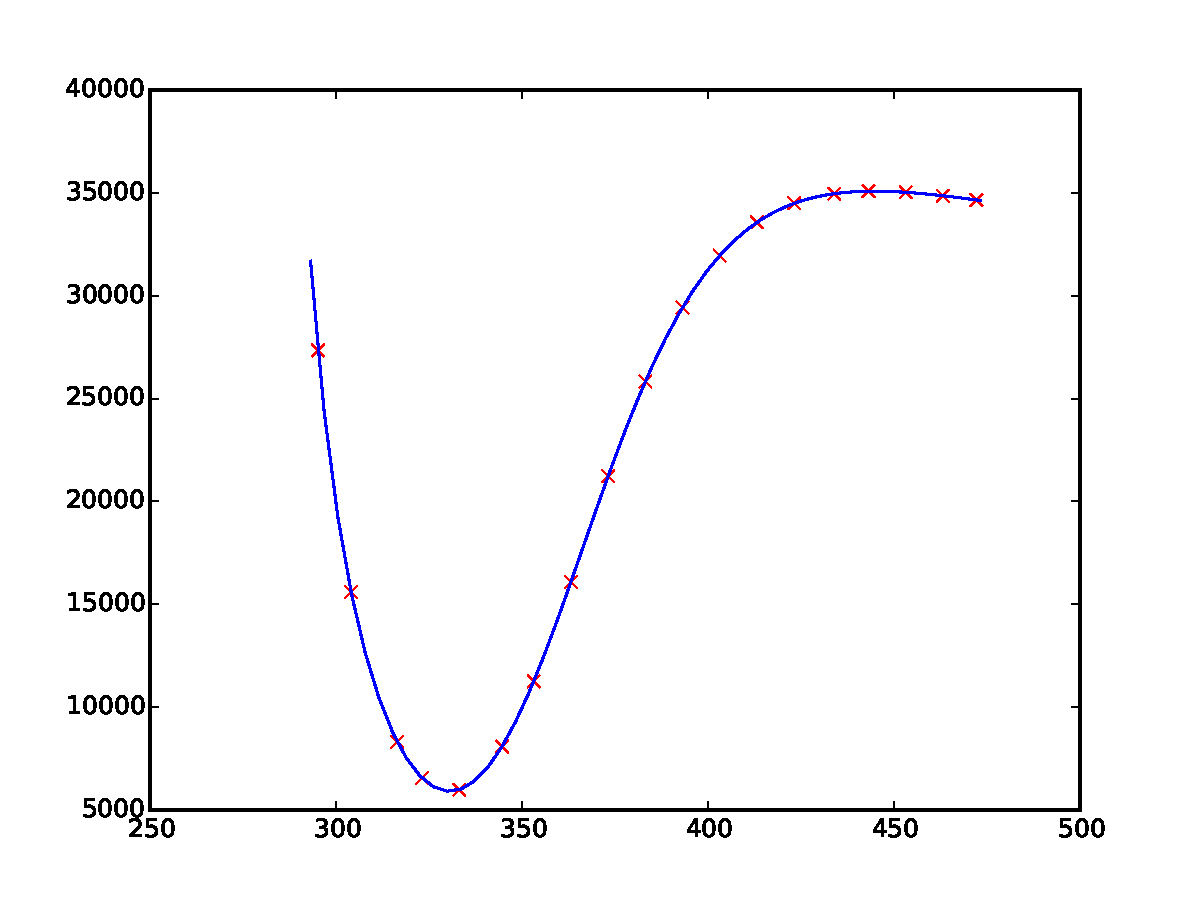
\includegraphics[width=0.7\textwidth]{plot4.pdf}
  \caption{Verdampfungswärme $L$ in Abhängigkeit von $T$ aus der Formel \eqref{eqn:L+} mit positivem Vorzeichen vor der Wurzel.}
  \label{abb:+}
\end{figure}
